\documentclass{article}
\usepackage[utf8]{inputenc}
\usepackage[margin=1in]{geometry} % Ajusta los márgenes a 1 pulgada
\usepackage{graphicx}
\usepackage{listings}
\usepackage{xcolor}
\usepackage{hyperref}

\definecolor{codegreen}{rgb}{0,0.6,0}
\definecolor{codegray}{rgb}{0.5,0.5,0.5}
\definecolor{codepurple}{rgb}{0.58,0,0.82}
\definecolor{backcolour}{rgb}{0.95,0.95,0.92}

\lstdefinestyle{mystyle}{
    backgroundcolor=\color{backcolour},
    commentstyle=\color{codegreen},
    keywordstyle=\color{magenta},
    numberstyle=\tiny\color{codegray},
    stringstyle=\color{codepurple},
    basicstyle=\ttfamily\small,
    breakatwhitespace=false,
    breaklines=true,
    captionpos=b,
    keepspaces=true,
    numbers=left,
    numbersep=5pt,
    showspaces=false,
    showstringspaces=false,
    showtabs=false,
    tabsize=2
}

\lstset{style=mystyle}

\title{Convolutional Neural Networks – Lab 5}
\author{RUBEN MARTINEZ GONZALEZ}
\date{\today}

\begin{document}

    \maketitle


    \section{introducción}\label{sec:introduccion}
    En este informe, se presenta el trabajo realizado en el laboratorio 5 de Redes Neuronales Convolucionales.
    Se implementaron varios bloques de código relacionados con el uso de la regresión lineal y el algoritmo de descenso de gradiente.
    Se ejemplificó el uso de la regresión lineal para predecir la altura de varios niños basándose en sus edades.

    \noindent
    La solución se implementó en Python utilizando la biblioteca TensorFlow para el aprendizaje, NumPy para el procesamiento de matrices y Matplotlib para la visualización de gráficos.
    La implementación está desplegada en un notebook de Google Colab, el cual se puede acceder a través del siguiente enlace:
    \texttt{%
        \href{https://colab.research.google.com/drive/1H1AKbWHVSPwCeDJuhiwpH5MEBkk3qcgb?usp=sharing}{%
            Colab}%
    }


    \section{Bloques de código implementados}\label{sec:bloques-de-codigo-implementados}

    \subsection{Plot your training data}\label{subsec:plot-training-data}
    En este bloque de código se grafican los datos de entrenamiento, donde se muestra la relación entre la edad y la altura de los niños.

    \begin{lstlisting}[language=Python, caption={Gráfica de los datos de entrenamiento},label={lst:PlotTrainingData}]
            import matplotlib.pyplot as plt

            # Load the data
            X_train = np.loadtxt('ex2x.dat')
            y_train = np.loadtxt('ex2y.dat')

            plt.scatter(X_train, y_train, marker='x', c='r')
            plt.title('Training Data')
            plt.xlabel('Age in years')
            plt.ylabel('Height in meters')
            plt.show()
    \end{lstlisting}
    \noindent
    Al ejecutar el código se obtuvo la siguiente gráfica:
    \begin{figure}[h]
        \centering
        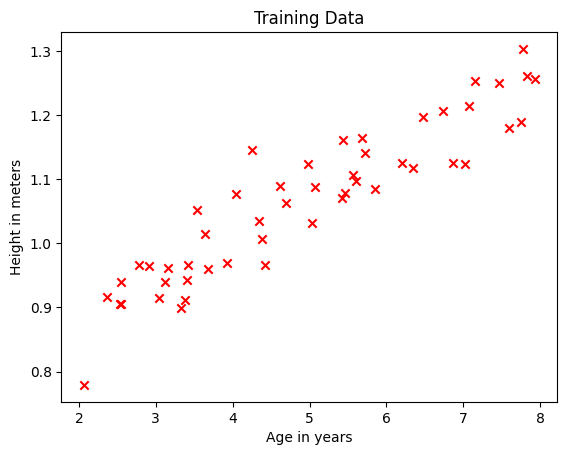
\includegraphics[width=0.8\textwidth]{img/plot_training_data}
        \caption{Gráfica de los datos de entrenamiento}
        \label{fig:plot_training_data}
    \end{figure}
    \clearpage

    \subsection{Linear Regression using Gradient Descent (TensorFlow)}\label{subsec:Gradient-Descent}
    \noindent
    En este bloque de código se implementa la regresión lineal utilizando el algoritmo de descenso de gradiente apoyado en la biblioteca TensorFlow.
    El objetivo de la implementación es poder predecir la altura de varios niños basándose en sus edades.
    Los valores de $x$ y $y$ se cargaron desde los archivos 'ex2x.dat' y 'ex2y.dat' respectivamente.

    \noindent
    La implementación realizada se describe a continuación:
    \begin{itemize}
        \item Se normalizaron los datos de entrada y salida.
        \item Se inicializaron las variables $m$ (número de ejemplos de entrenamiento),
        $\alpha$ (tasa de aprendizaje = 0.1) y
        $\theta$ (parámetros iniciales aleatorios con distribución normal).
        \item Se definió la función de hipótesis $h_{\theta}(x) = \theta_0 + \theta_1 * x$.
        \item Se definió la función de costo (error cuadrático medio)
        $J(\theta) = \frac{1}{2m} \sum_{i=1}^{m} (h_{\theta}(x^{(i)}) - y^{(i)})^2$.
        \item Se definió el optimizador (descenso de gradiente estocástico).
        \item Se ejecutó una iteración del algoritmo de descenso de gradiente.
    \end{itemize}
    \noindent
    Al ejecutar el código se obtuvieron los siguientes resultados:
    \begin{itemize}
        \item Cost after 1 iterations: 3.884464
        \item Theta0 after one iteration: tf.Tensor([-0.09925186], shape=(1,), dtype=float32)
        \item Theta1 after one iteration: tf.Tensor([-0.34086537], shape=(1,), dtype=float32)
    \end{itemize}
    \begin{lstlisting}[language=Python, caption={Regresión lineal utilizando descenso de gradiente},label={lst:GradientDescent}]
# Normalize the input data
X_mean = np.mean(X_train)
X_std = np.std(X_train)
X_train = (X_train - X_mean) / X_std

# Normalize the output data
y_mean = np.mean(y_train)
y_std = np.std(y_train)
y_train = (y_train - y_mean) / y_std

# Initialize variables
m = len(X_train)      # Number of training examples
alpha = 0.1          # Learning rate
theta = tf.Variable(tf.random.normal([2, 1]), dtype=tf.float32) # Initial random parameters

# Define the model
def hypothesis(X):
    return theta[0] + theta[1] * X

# Define the cost function (mean squared error)
def cost_function(X, y):
    return tf.reduce_mean(tf.square(hypothesis(X) - y))

# Define the optimizer
optimizer = tf.keras.optimizers.SGD(learning_rate=alpha)

with tf.GradientTape() as tape:
    cost = cost_function(X_train, y_train)
    gradients = tape.gradient(cost, [theta])
    optimizer.apply_gradients(zip(gradients, [theta]))
    print("Cost after", 1, "iterations:", cost.numpy())
    print('Theta0 after one iteration:', theta[0])
    print('Theta1 after one iteration:', theta[1])
    \end{lstlisting}
    \clearpage

    \subsection{Continue running gradient descent for more iterations}\label{ssec:Continue-Running-Gradient-Descent}
    En este bloque de código se ejecutan 200 iteraciones del algoritmo de descenso de gradiente.
    \begin{lstlisting}[language=Python, caption={Ejecución de 200 iteraciones del algoritmo de descenso de gradiente},label={lst:ContinueRunningGradientDescent}]
# Perform gradient descent
for i in range(300):
    # Perform one step of gradient descent
    with tf.GradientTape() as tape:
        cost = cost_function(X_train, y_train)
    gradients = tape.gradient(cost, [theta])
    optimizer.apply_gradients(zip(gradients, [theta]))

    # Print cost every 50 iterations
    if i % 50 == 0:
        print("Cost after", i, "iterations:", cost.numpy())

# Get the learned parameters
final_theta = theta.numpy()
print('Final Theta:', final_theta.ravel())
    \end{lstlisting}
    \noindent
    Al ejecutar el código se obtuvieron los siguientes resultados:
    \begin{itemize}
        \item Cost after 0 iterations: 1.7575389
        \item Cost after 50 iterations: 0.14193676
        \item Cost after 100 iterations: 0.14193676
        \item Cost after 150 iterations: 0.14193676
        \item Final Theta: [1.3125225e-08 9.2631692e-01]
    \end{itemize}

%After convergence, plot the straight line fit from your algorithm on the same graph as your training data.

    \subsection{Plot the straight line fit from your algorithm}\label{ssec:Plot-Straight-Line-Fit}
    En este bloque de código se grafica la línea recta ajustada por los parámetros aprendidos por el algoritmo de descenso de gradiente
    junto a los datos de entrenamiento. Se muestra la relación entre la edad y la altura de los niños.

    \begin{lstlisting}[language=Python, caption={Gráfica de la línea recta ajustada por el algoritmo de descenso de gradiente},label={lst:PlotStraightLineFit}]
# Plot the training data and the fitted line
plt.scatter(X_train, y_train, marker='x', c='r', label='Training Data')
plt.plot(X_train, final_theta[0] + final_theta[1] * X_train, color='b', label='Fitted Line')
plt.title('Training Data with Fitted Line')
plt.xlabel('Age in years (normalized)')
plt.ylabel('Height in meters (normalized)')
plt.legend()
plt.show()
    \end{lstlisting}
    \noindent
    Al ejecutar el código se obtuvo la siguiente gráfica:
    \begin{figure}[h]
        \centering
        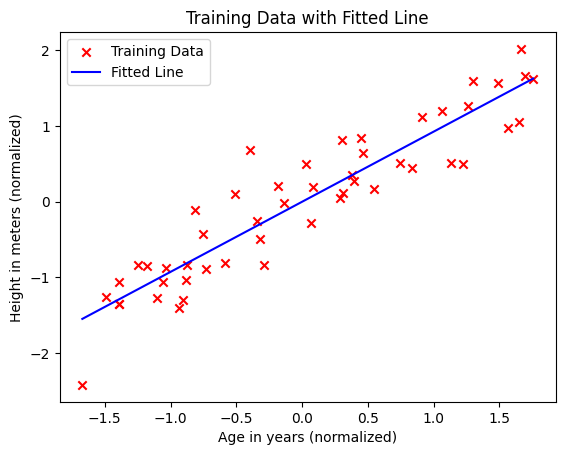
\includegraphics[width=0.8\textwidth]{img/plot_straight_line_fit}
        \caption{Gráfica de la línea recta ajustada por el algoritmo de descenso de gradiente}
        \label{fig:plot_straight_line_fit}
    \end{figure}
    \clearpage

    \subsection{Use your trained model to predict height   }\label{ssec:Predict-Height}
    En este bloque de código se utilizan los parámetros aprendidos por el algoritmo de descenso de gradiente para predecir la altura de dos niños de 3.5 y 7 años.
    \begin{lstlisting}[language=Python, caption={Predicción de la altura de dos niños de 3.5 y 7 años},label={lst:PredictHeight}]
# Predict heights for boys of age 3.5 and 7
age_3_5_height = theta[0] + theta[1] * 3.5
age_7_height = theta[0] + theta[1] * 7

# Print the predicted heights
print('Predicted height for a boy of age 3.5:', round(age_3_5_height,2))
print('Predicted height for a boy of age 7:', round(age_7_height,2))
    \end{lstlisting}
    \noindent
    Al ejecutar el código se obtuvieron los siguientes resultados:
    \begin{itemize}
        \item Predicted height for a boy of age 3.5: 0.97
        \item Predicted height for a boy of age 7: 1.2
    \end{itemize}

    \clearpage


    \section{Conclusiones}
    \noindent
    En este informe se presentó el trabajo realizado en el laboratorio 3 de Redes Neuronales Convolucionales.
    Se implementaron varios bloques de código relacionados con el uso de la regresión lineal y el algoritmo de descenso de gradiente.
    se ejemplificó el uso de la regresión lineal para predecir la altura de varios niños basándose en sus edades.
    Se utilizó una tasa de aprendizaje de $\alpha = 0.07$ y se realizaron 1000 iteraciones del algoritmo de descenso de gradiente.
    Se graficaron los datos de entrenamiento y la línea recta ajustada por los parámetros aprendidos por el algoritmo de descenso de gradiente.
    Se utilizó el modelo entrenado para predecir la altura de dos niños de 3.5 y 7 años.

\end{document}
